\documentclass[10pt,a4paper]{article}


% Packages laden
\usepackage[a4paper,top=3cm,bottom=2cm,left=2cm,right=2cm]{geometry}		% paginagrootte
%\usepackage{a4wide}
\usepackage{parskip}									% andere regels voor nieuwe paragraaf: witregel + niet inspringen

\usepackage[english]{babel}						%	spelling en woordafbreking (Engles)
\usepackage[latin1]{inputenc}					% invoer van speciale tekens (bvb. Umlaut)
\usepackage[T1]{fontenc}							% weergave van speciale tekens (bvb. Umlaut)
\usepackage{lmodern}									% betere weergave van speciale tekens (bvb. Umlaut)
%\usepackage{dsfont}	
\usepackage{amsfonts,amsthm, tabularx}					% wiskundige symbolen and table of equations
%\usepackage[fleqn]{amsmath}
\usepackage{graphicx}
\usepackage{epstopdf}

% Package for hyperlink, without ugly box around and nice blue color for text
\usepackage{hyperref}
\usepackage{xcolor}
\hypersetup{
    colorlinks,
    linkcolor={red!50!black},
    citecolor={blue!50!black},
    urlcolor={blue!80!black}
}

\usepackage{graphicx}
\usepackage{caption}
\usepackage{subcaption}

\usepackage{float}										% plaatsen van figuren en tabellen
\usepackage[format=plain,
						indent=1cm]{caption}			% personaliseren van onderschriften
\usepackage{eurosym}									% sign of euro

% Instellingen voor document
\renewcommand{\arraystretch}{1.1}			% tabelrijen iets hoger maken

\usepackage[squaren,Gray]{SIunits}
\usepackage{amsmath,amsfonts,amsthm,mathrsfs,MnSymbol}	% wiskundige symbolen
\renewcommand*\thesection{\arabic{section}}
\DeclareMathOperator*{\argmin}{\arg\!\min}
\usepackage{pifont}							

\setcounter{secnumdepth}{3}		% Enable subsubsection numbering
\setcounter{tocdepth}{3}		% Include subsubsection in table of content

\usepackage{color}				% Load the color package: \color{declared-color}{text}. If also background:
								% \colorbox{declared-color1}{\color{declared-color2}text}
%Aangepaste header
\usepackage{fancyhdr}
\pagestyle{fancyplain}
\renewcommand{\headrulewidth}{1.0pt}
\lhead{\fancyplain{}{Crash course Modelica}}
\rhead{\fancyplain{}{\today}}

\author{Damien Picard}
						
\begin{document}

\section*{Prepare for the Modelica Crash Course!}

This guide will help you to install Dymola and already get the hang of Modelica, such that you can profit maximally from the Crash Course. 

\subsection*{Installation}

First of all, install Dymola (commercial software).  Fill out this 
\href{http://www.claytex.com/products/dymola/dymola-demo/}{form} to download 
the demo. After installation you HAVE to install a c-compiler, otherwise you 
cannot run any model.  You can download and install for example the Visual 
Studio \texttt{C++} 2015 Build Tools from this  
\href{http://landinghub.visualstudio.com/visual-cpp-build-tools}{link}. 
Do not forget to select your C-compiler in Dymola>Simulation Set Up>Compiler. 
In order to access this menu item, open Dymola and change to the Simulation tab 
(lower right corner).
Test your installation by running a demo (e.g. open File/Demos/Robot, then 
click Commands/Simulate and wait till you see a graph). 
More detailed 
instructions can be found 
\href{https://www.3ds.com/fileadmin/PRODUCTS/CATIA/DYMOLA/PDF/Installation.pdf}{here}.

\subsection*{Prerequisites}
Read the following chapters of the open-access book  
\href{http://book.xogeny.com/}{Modelica by Example} of Michael M. Tiller 
carefully.
If the website is offline, refer to the pdf version on \href{https://github.com/open-ideas/__CrashCourse__/blob/master/2017-2018/ModelicaByExample.pdf}{GitHub}. The website offers the advantage of interactive examples of Modelica code.

\begin{enumerate}
\item \href{http://book.xogeny.com/behavior/equations/}{Basic equations}: general introduction to the Modelica language, illustration of the model structure, basic concepts such as derivative, initialization, parameter, variable and type.
\item \href{http://book.xogeny.com/behavior/functions/polynomial/}{Polynomial Evaluation}: introduction to function definition, protected variable and time.
\item \href{http://book.xogeny.com/behavior/arrays/oned/}{One-Dimensional Heat Transfer}: introduction to arrays and loop in Modelica.
\item	\href{http://book.xogeny.com/components/connectors/}{Connectors}: Component-Oriented Modeling, classes of variables.



\end{enumerate}

Read carefully chapter 1 ``What is Dymola?'', p.~13 to 22, of the Dymola manual Volume 1 (can be found in your installation folder: C:\textbackslash Program Files (x86)\textbackslash Dymola \textit{xx}\textbackslash Documentation \textbackslash Dymola User Manual Volume 1, where \textit{xx} stands for the version you installed) to get familiar with the Dymola environment (model editor, parameters change, simulation, ...).\\

Additionally, to come prepared for the course, please read through the following parts of ``Modelica by Example'' of Michael Tiller: 
\begin{enumerate}
\item \href{http://book.xogeny.com/behavior/discrete/}{Discrete Behavior} >State Event Handling, Hysteresis and Review
\item	\href{http://book.xogeny.com/behavior/arrays/}{Vectors and Arrays} >Array Declarations and Array Construction
\item	\href{http://book.xogeny.com/components/components/#review}{Components}>Review, Examples>Heat Transfer Components, Electrical Components
\item \href{http://book.xogeny.com/components/architectures/replaceable/}{Architecture>Configuration Management}
		
\end{enumerate}

\subsection*{Homework exercise}
The purpose of this exercise is to model an electrical circuit using only your own code implementation. You will learn how to create connectors, partial models, models and how to re-use your code.

\begin{figure}[h]
	\centering
	\begin{minipage}{.4\textwidth}
		\centering
		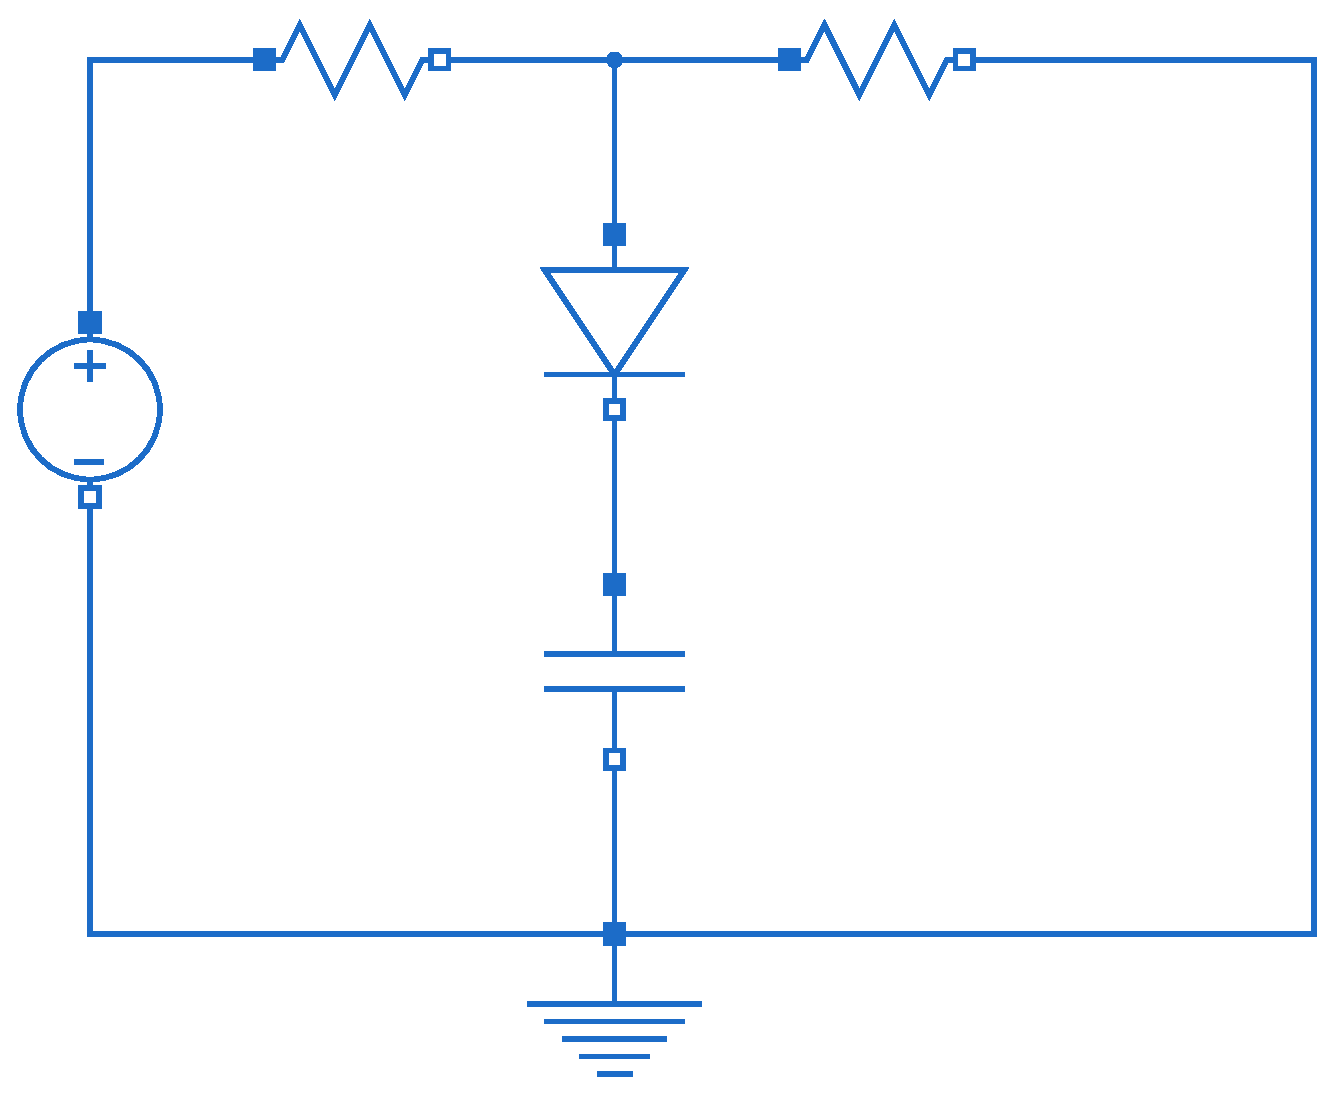
\includegraphics[width=1\linewidth]{images/circuit.eps}
		\captionof{figure}{Electrical circuit.}
		\label{fig:cir}
	\end{minipage}%
	\begin{minipage}{.6\textwidth}
		\centering
		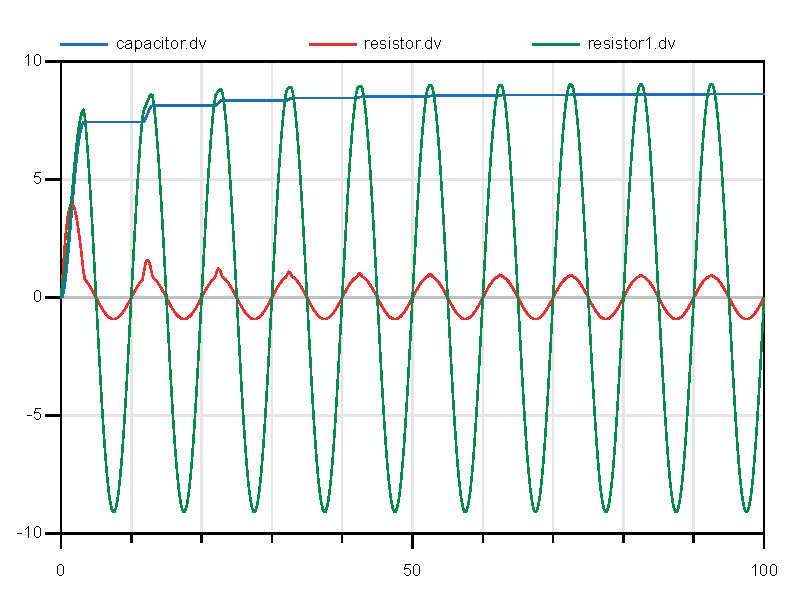
\includegraphics[width=.8\linewidth]{images/result.eps}
		\captionof{figure}{Result of simulation}
		\label{fig:res}
	\end{minipage}
\end{figure}


Consider the electrical circuit shown in Fig.~\ref{fig:cir}. The circuit has a sinusoidal source, a resistor, a diode, a capacitor and the ground. You are going to build your first Modelica library from scratch to compose this model.


\begin{enumerate}
	\item After opening Dymola, create a new \textit{package} called \textit{MyLib}. All component models you will define in the following step need to be placed in this folder.
	
	\item Each component uses electrical connectors. Create a \texttt{partial connector} called \textit{Pin} which contains the variables $i$ (current) and $v$ (voltage). You can add variables while you are in the \textit{Modelica text} context of the \textit{Modeling} tab. Which one is a \textit{flow} and which is a \textit{potential} variable, and how should this be reflected in your code? 
	
	\item Create the \texttt{connector}s \textit{Pin\_a} and \textit{Pin\_b} for the positive and negative pins. Make two different graphical illustrations for the pins. Use \texttt{extends} to inherit the variables $i$ and $v$ from the \texttt{partial connector} you have just defined. An easy way to create extending models is by right-clicking on the model you want to extend from, and click \textit{New > Extend from\ldots}.
	
	\item Create a \texttt{partial model} \textit{OnePin} which contains the variables $i$ (current) and $v$ (voltage) and one connector \textit{Pin\_a}. To add the connector, drag \textit{Pin\_a} from your libary folder to the modelling window while you are in the \textit{Diagram} context of the \textit{Modeling} tab. The pin should be located at the top border of the white box. This model will be the basis for all models which have only one pin (i.e., the ground node).
	
	\item Create variables $i$ and $v$ in \textit{OnePin} and write \texttt{equation}s to link these variables to those you have defined in the \textit{Pin} you use in the component. In order to access variables, you can use dot notation as follows: \texttt{componentName.variable}. 
	
	\item Now create a \texttt{partial model} \textit{TwoPin} with the same variables and two \textit{Pin} connectors, one positive pin on the left and one negative on the right. Add two variables: voltage difference $dv$ and current $i$. 
	While still in \texttt{partial model} \textit{TwoPin}, add equations that link the variables in this model with the variables of the pins. When connecting currents, use the convention that when the current flows into the component from the pin, it is positive and vice versa.
	
	\item Create the source, the resistor, the diode and the capacity by extending \textit{OnePin} or \textit{TwoPin}. Make use of the following equations:
	\begin{enumerate}
		\item Resistor: $R i = v$\footnote{$v$ in this equation is equivalent to variable $dv$ in the Modelica model.}
		\item Capacity: $C \frac{d v}{dt} = i$
		\item source: $v = V sin( 2 \pi f t + \omega) + \beta$
		\item Diode: if $ \frac{v}{V_t} \geq \alpha$: $i = I_{ds} \left( \exp\left(\alpha \left( 1 + \frac{v}{V_t} - \alpha \right)\right) - 1\right) + \frac{v}{R}$, else $i = I_{ds} (e^\alpha - 1) + \frac{v}{R}$
		\item ground: $ v = 0$
	\end{enumerate}
	Define $R$, $C$,\ldots as \texttt{parameter}, such that you can change their value using the parameter dialog in the \textit{Diagram} context.\\
	Make use of following values for the diode: $I_{ds}$ = 1.e-6, $V_t=0.04$, $\alpha=1$, $R=1.e8$.
	\item Create a model called \textit{Circuit} in which you include all these components as shown in Fig.~\ref{fig:cir}.
	\item Simulate the circuit for 100 seconds.
\end{enumerate}

\subsection*{Optional exercise}
This assignment aims at testing your comprehension of the basic Modelica concepts learned during the above mentioned reading by setting a model of a building and simulating its thermal behaviour. \textbf{This assignment will not be treated during the Crash Course. However, you may find it a useful exercise to get more acquainted with Modelica and Dymola.}

Let us consider a simplified building as represented in Fig. \ref{fig:bui}. The building consists of  walls, a window and a single room called \textit{zone} which thermally interacts with the environment(ambient air \textit{TAmb}, the ground, and the sun. The building foundation is approximated by a thick concrete layer called \textit{slab} separating the zone from the ground. On the right-hand side of the figure, a thermal model of the building is proposed using the resistance-capacitance approach. The heat transfer is approximated by a 1D conduction resistance and the heat storage by a heat capacity. \textit{CZone} represents the thermal capacity of the zone (consisting of the internal walls, the furnitures, and a part of the external wall). The \textit{CSlab}'s represent the thermal capacities of the slab. Finally, the ground is discretized in \textit{n = 5} layers, each of them having an identical heat capacity \textit{CGro[i]}. Through the window, the sun heats up the room with a thermal power $QSol$. 

The value of the parameters is given in Table \ref{tab:par}. Using the electrical analogy, the governing equations of the system are the following:

\begin{figure}[hbtp] 
	\centering
	\includegraphics[width=1 \textwidth]{images/RCModelHouse.pdf}
	\caption{ Building model.}
	\label{fig:bui}
\end{figure}

\begin{table}[hbtp] 
\begin{tabular}{cccccc}
\hline 
  & RWall & RSlab1 & RSlab2 & RGro1[i] & RGro2[i] \\  
Thermal resistance $[K/W]$ & 0.00806 & 0.016 & 0.016 & 0.033 & 0.033 \\ 
\hline\hline 
  & CZone & CSlab & CGro[i] &   &   \\  
Thermal capacities $[J/K]$ & $2.4096 * 10^8$ & $3.36 * 10^8$ & $2.52*10^8$ &   &   \\ 
\hline\hline
  & TGroIni & TGro[i](start) & TSlab(start) & TZone(start)&  \\  
Temperature $[K]$ &  283.15 & 283.15 & 293.15 & 293.15 & \\ 
\hline 
\end{tabular} 
\caption{ Building parameters.}
\label{tab:par}
\end{table}

%\newpage
\textbf{Thermal resistance}: $T_1 - T_2 = \text{R} \ Q_{1 \rightarrow 2} $ with $R$ the thermal resistance between node 1 and 2 and $Q_{1\rightarrow 2}$ the heat flow, positive defined from 1 to 2.

\textbf{Thermal capacity}: $C \frac{\text{dT}}{dt} = Q$ with $C$ the thermal capacity and $Q$ the heat flow, positive defined flowing to the capacity.

\textbf{Conservation of energy (Kirchhoff)}: $ \sum Q_i = 0$ or the sum of the heat flows through one node is zero.

\subsection*{Questions}

\begin{enumerate}
\item Apply what you have learned during your reading by setting up a model for the building using the above mentioned equations. Approximate the ambient temperature by a sine using following code: $TAmb = 10*\cos(2*3.14*\text{time}*3*10^\wedge(-8)) + 276.15$ and the solar radiation by a trimmed cosine using: $QSol = \text{floor}(cos(2*\text{Modelica.Constants.pi}*\text{time} / 86400) + 1) * 5000 * cos(2*\text{Modelica.Constants.pi*time} / 86400)$. What is the zone temperature after a year under these conditions?
\item (OPTIONAL): Try to obtain the same results using the components of the Modelica library instead of writting the equations yourself. This library is automatically loaded in Dymola and can be found on the left-hand side of the dymola window. For thermal components, look in the Library at Modelica.Thermal.HeatTransfer.Components.   \linebreak[10]
\end{enumerate}

\begin{center}
 \textbf{Good luck!}
\end{center}

\subsection*{Further reading}
\begin{itemize}
	\item \url{http://simulationresearch.lbl.gov/modelica/downloads/workshops/2015-06-22-lbnl/slides/modelica-intro.pdf}
	\item \url{http://book.xogeny.com}
\end{itemize}

\end{document}
